\chapter{Methodology}
\label{ch:methodology}

In this chapter it will be explained how the cluster analysis and the experiments were conducted. The first part of the chapter is dedicated to define some concepts related to the On Target product: the OT itself and its benchmark project. The second part is about the cluster analysis. And the third one is about the experiments.

\section{About the Product}

Before getting to the clustering and experiment procedures, it is important to define some concepts about the OT product. A high level explanation of the OT and how its benchmark was built will be described in this first part of the chapter.

\subsection{On Target}

The On Target is one of the Neoway's products of the vertical of Sales and Marketing. It is a content-based recommender system that searches for leads based on the customers' profile of the user. The OT receives as input:
\begin{itemize}
    \item the \textbf{Portfolio}, which is the list of companies that are customers of the OT user. It can range from a few dozens to dozens of thousands companies;
    \item the \textbf{Market}, which is the list of companies where the OT will search for the leads. It can range from dozens to tens of millions companies; and
    \item the \textbf{Features}, which is a data set with the characteristics of the companies.
\end{itemize}
And it outputs the sorted \underline{Market} based on a score called \textbf{Similarity}. Figure \ref{fig:ot-blocks} illustrates a block diagram of the OT.

\begin{figure}[h]
   \centering
   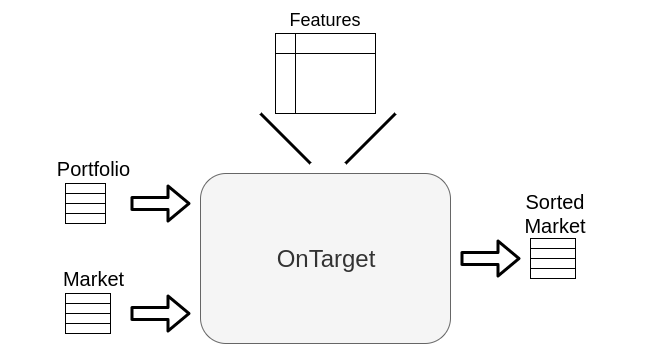
\includegraphics[width=\linewidth]{fig/ch3-ot-blocks.png}
   \caption{Block Diagram of the On Target. Source: Author}
   \label{fig:ot-blocks}
\end{figure}

\subsection{Benchmark}

As mentioned on the chapter \ref{ch:introduction}, the recommender system was update and one of the ways to assure that the modifications had a positive impact on the algorithm was to develop a benchmark. The Benchmark is a project that compares different versions of the OT, by running these versions on almost thirty different business scenarios. They can be: one retail customer with a huge portfolio and huge market size; or a bank with a small portfolio and medium market size; or even a service provider with small portfolio and small market size. A run of the OT for one of this scenarios is called a \textbf{Study}. An \textbf{Experiment} is the run of all of these scenarios for new versions of the OT comparing to the current one that it is running on production. Every modification on the algorithm generates a new experiment. For instance, if the number of features is increased, an experiment (or more) is generated. If a parameter of the algorithm is changed, a new experiment is generated.

The Benchmark does some minor modification on the OT pipeline. It removes a random sample of companies from the portfolio (it can be 10\%, 30\% or 50\%) and it places them on the market. The idea is to use this sample as holdout set \cite{kohavi2001}, which is a separated part of the data used for test. For the OT these companies are in the market, without "knowing" that they came from the portfolio, therefore it is expected that the companies in the holdout set have a high score (similarity) on the output. Figure \ref{fig:ot-benchmark-blocks} shows these modifications on the OT.

\begin{figure}[h]
   \centering
   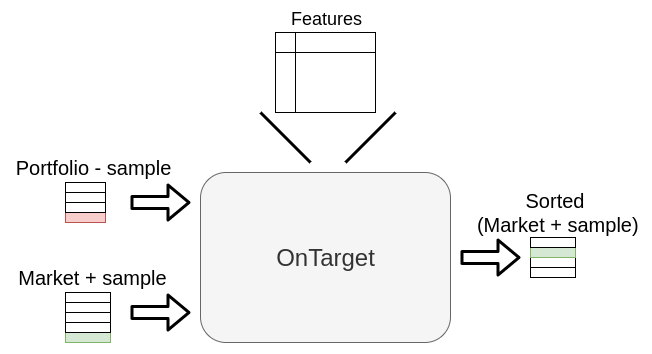
\includegraphics[width=\linewidth]{fig/ch3-ot-benchmark-blocks.png}
   \caption{Modifications on the OT done by the Benchmark. Source: Author}
   \label{fig:ot-benchmark-blocks}
\end{figure}

These changes on the pipeline are to generate the metrics to evaluate the experiments in two ways. The first one, is the performance with the \textbf{lift}, usually only the first decile, but there is a plot, also. The second one is consistency, with the \textbf{similarity distribution} plot. On the former, the holdout set is used to calculate the probabilities after the sorting of the OT - similar to the red balls analogy discussed on \ref{ch:evaluation}. The latter, plots the distribution of the scores assigned to the market and to the holdout set. As seen on the Introduction chapter of this work, Figure \ref{fig:simi-dist-expected-real} shows an example of this plot, where the orange are the holdout set and the blue curve is the market.

\section{Cluster analysis}

In this seconds part of the chapter it will be explained how the clusters analysis were conducted. It will be explained how and what are the clustering strategies and clusters pairing. Also, a discussion about definition of number of clusters and the choice of the cluster algorithm.

\subsection{Clustering strategy and pairing}

The first thing to tackle was the definition of the clustering strategy and pairing. The strategy of how the cluster algorithm will be applied on the data and how the clusters from the portfolio will be paired with the clusters from the market. 

Basically, for the strategy, there are two possible ones: \textit{training the cluster algorithm on the portfolio and applying it on the market} (\textbf{clustering strategy I}) or \textit{training and applying on all the data} (\textbf{stra-tegy II}). Let us take the example of the KMeans algorithm using these two strategies applied on a fake study dataset, which is illustrated on Figure \ref{fig:cluster-strategy}. Assuming that all sub plots are on the same scale, in (I) we see the portfolio clustered with its two centroids, on (II) we can see the KMeans "predicting"\footnote{this is a fairly common name for the inference step of an algorithm in scikit-learn implementation} the clusters of all data with the centroids learned on (I). This is the \textbf{clustering strategy I}. The \textbf{clustering strategy II} is represented on (III) where the KMeans trains and predicts on all data. We can see that the centroids are on different positions, as a result some companies are allocated on a different cluster relative to (II). 

\begin{figure}[h]
   \centering
   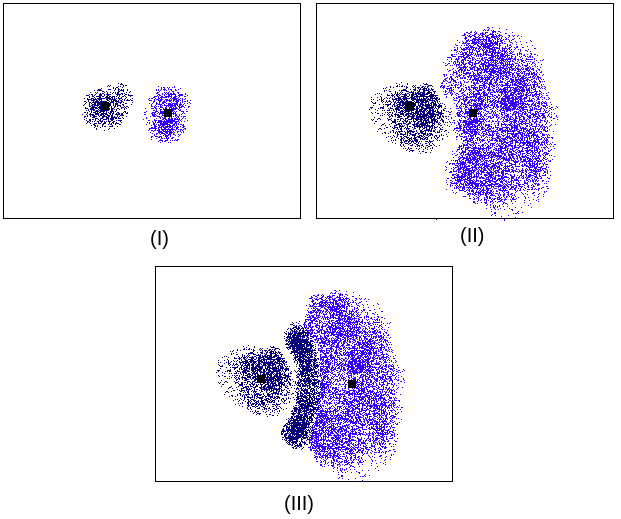
\includegraphics[width=9cm]{fig/ch3-cluster-strategy.png}
   \caption{Fake study data set that shows how both clustering strategies work. Source: Author}
   \label{fig:cluster-strategy}
\end{figure}

For the pairing there are also two possible ways: \textit{each cluster on the portfolio will be matched with its cluster on the market} (\textbf{cluster pairing I}) or \textit{each cluster on the portfolio will run with the whole market} (\textbf{cluster pairing II}). For instance, if we have a study that have three clusters on the portfolio with 50 companies each, and 150 companies on each cluster on the market, in \textbf{cluster pairing I} the OT will run three times with a portfolio size of 50 and market size of 150; for \textbf{cluster pairing II} the OT will run three times with a portfolio size of 50 and a market size of 450 (whole market for each cluster). Figure \ref{fig:cluster-pairing} shows a block diagram of this scenario.

\begin{figure}[h]
   \centering
   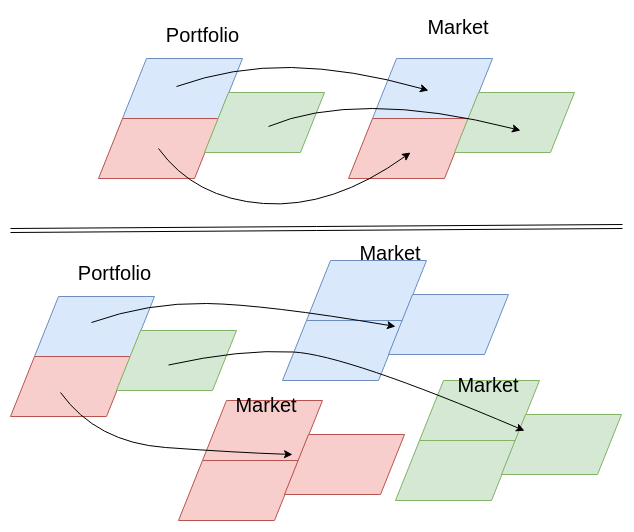
\includegraphics[width=7cm]{fig/ch3-cluster-pairing.png}
   \caption{Illustration of the cluster pairing. On the top is the cluster pairing (I) and on the bottom the cluster pairing (II). Source: Author}
   \label{fig:cluster-pairing}
\end{figure}

Through a business view, it makes more sense to adopt the \textbf{clustering strategy I} since we are interested on the recommendations based on the user profile, in other words, the user's portfolio, regardless of the market data. 

On cluster pairing II the market is replicated for each cluster, leading each company to be scored N times (N being the number of clusters). Hence, there could be cases where one company has a high score in a cluster while, at the same time, have a low score in other one. To not deal with these cases the \textbf{cluster pairing I} was chosen for this work.

\subsection{Number of clusters}

The second aspect of the cluster analysis was the number of clusters for each study, since most of the cluster algorithms need this information upfront. Even though, there are some research on evaluating the number of clusters automatically \cite{yu2014automatic}, there are no production-ready solutions. There are, however, methods like Elbow method and Silhouette \cite{kodinariya2013review} that help with the determination of the number of clusters, but they are not reliable 100\% of the time, meaning that it would be difficult to automate. Considering that the objective is to analyse the impact of the clustering on the RS and not the cluster analysis itself and that there are only up to thirty studies, it was decided to set the number of the clusters \textbf{manually}.

To visualize the clusters on the studies, it is necessary to plot the data. But OT uses too many variables on production to analyse all of it at once. Hence, it was applied PCA transformation on the studies and used the first two principal components to plot the transformed data and to see the patterns in it. 

Before applying the PCA, a preprocessing step was needed. Categorical features were converted to numeric using One Hot Encoding and all features were scaled using the Z-score Normalization\footnote{all of the data transformations functions used on this theses are from the Scikit-learn Python library \cite{scikit-learn}}.

Figure \ref{fig:pca-plot} shows the results of the PCA plot for some studies using all features that OT uses on production environment (top), and PCA plot using only firmographics features for the sames studies (bottom). Each study is a column, where the first row is the plot of the PCA for the portfolio data, the second row the PCA plot for the market data, and the third row is for both, using different colors to distinguish portfolio from market (blue is the market and orange the portfolio).

We can see that it is much more difficult to visualise the clusters on the all-features PCA plot. There are some examples where you see a clear boundary on the data, but if wee look to the firmographics plot these boundaries are much more defined. Moreover, if you take to account the business perspective, it makes sense to group the companies by their firmographics. For example, a study with one clusters with big companies from the state of São Paulo and the other one with small companies from the state of Santa Catarina.

Using the firmographics PCA plot, each study was assigned with a number of clusters manually. For instance, on Figure \ref{fig:pca-plot}, from left to right, the number of clusters in the portfolio assigned are, respectively: 3, 3, 3, 2, 4, 3, 2, 2.  

\begin{figure}[h]
   \centering
   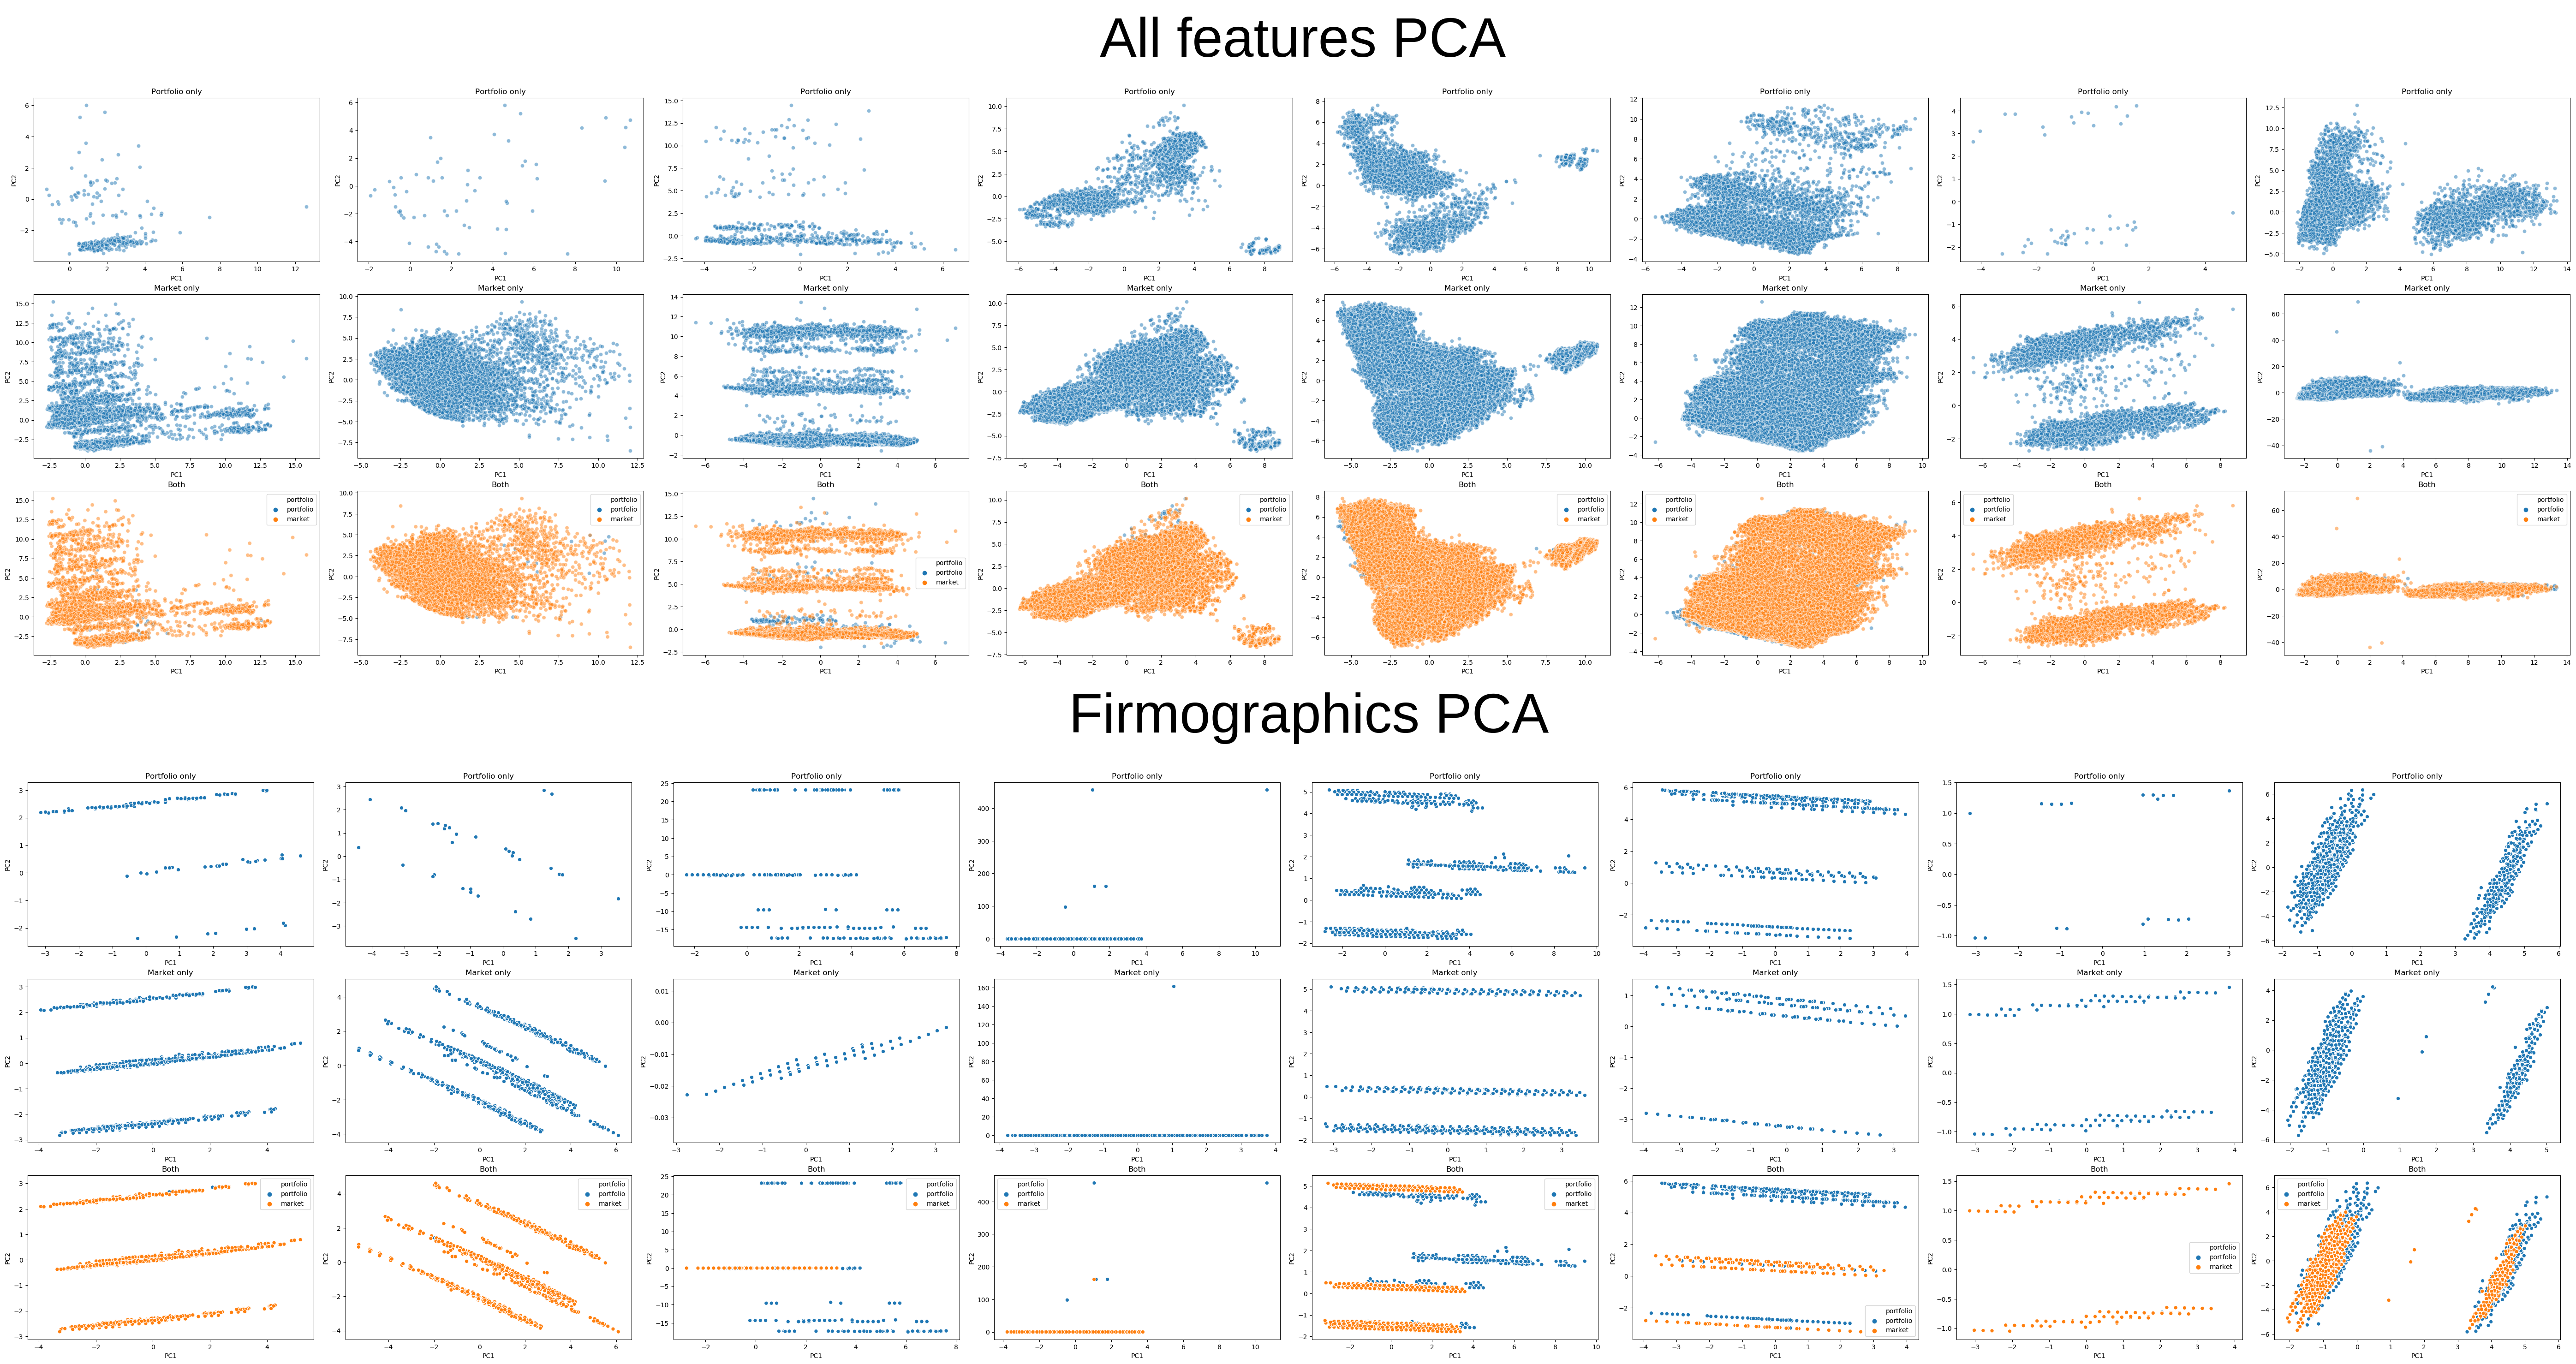
\includegraphics[width=\linewidth]{fig/ch3-pca-plot.png}
   \caption{PCA plot for the studies. On the top there is the the one using all features and on the bottom, only using firmographics features. Source: Author}
   \label{fig:pca-plot}
\end{figure}

\subsection{Cluster algorithm}

The last aspect of the cluster analysis was the choice of the algorithm. From the firmographics two principal components data, six clusters algorithms were applied on all the studies: \underline{KMeans}, \underline{Gaussian Mixture}, \underline{Bayesian Gaussian Mixture}, \underline{Agglomerative Clustering}, \underline{Spectral Clustering}, \underline{DBSCAN}\footnote{all of these implementations came from the scikit-learn python library \cite{scikit-learn}}. All of them were computed with default parameters and the same seed.

The latter three did not run on some studies that have a market size in an order of magnitude of dozen of thousands companies, due to memory error\footnote{all the algorithms were running on a machine with 250 GB of RAM}. Because of their high memory complexity \cite{franti2006fast}, \cite{ester1996density}, \cite{yan2009fast}, they were discarded.

The studies were also clustered \underline{manually} in order to be used as a benchmark for the algorithms. "Manually" in a sense that the boundaries among the clusters were defined without an algorithm. Since, most of the PCA plots present a regression characteristic, these boundaries were lines equations. Figure \ref{fig:clustering-studies} shows the results for some of the studies using "Manual Clustering", KMeans, Gaussian Mixture (GMM) and Bayesian Gaussian Mixture (BayesianGM).

As we can see the algorithms did not get the shape of the data in some of the studies. The Bayesian and GMM had better results relative to the KMeans. But they did not assigned the clusters as expected, for instance, on the third and sixth row of Figure \ref{fig:clustering-studies}. Due to these reasons and the same argument explained on the number of clusters discussion - we are interested on the results on the RS and not in the cluster analysis itself - it was decided by the team to start to the experiments using the "Manual Clustering".

\begin{figure}[H]
   \centering
   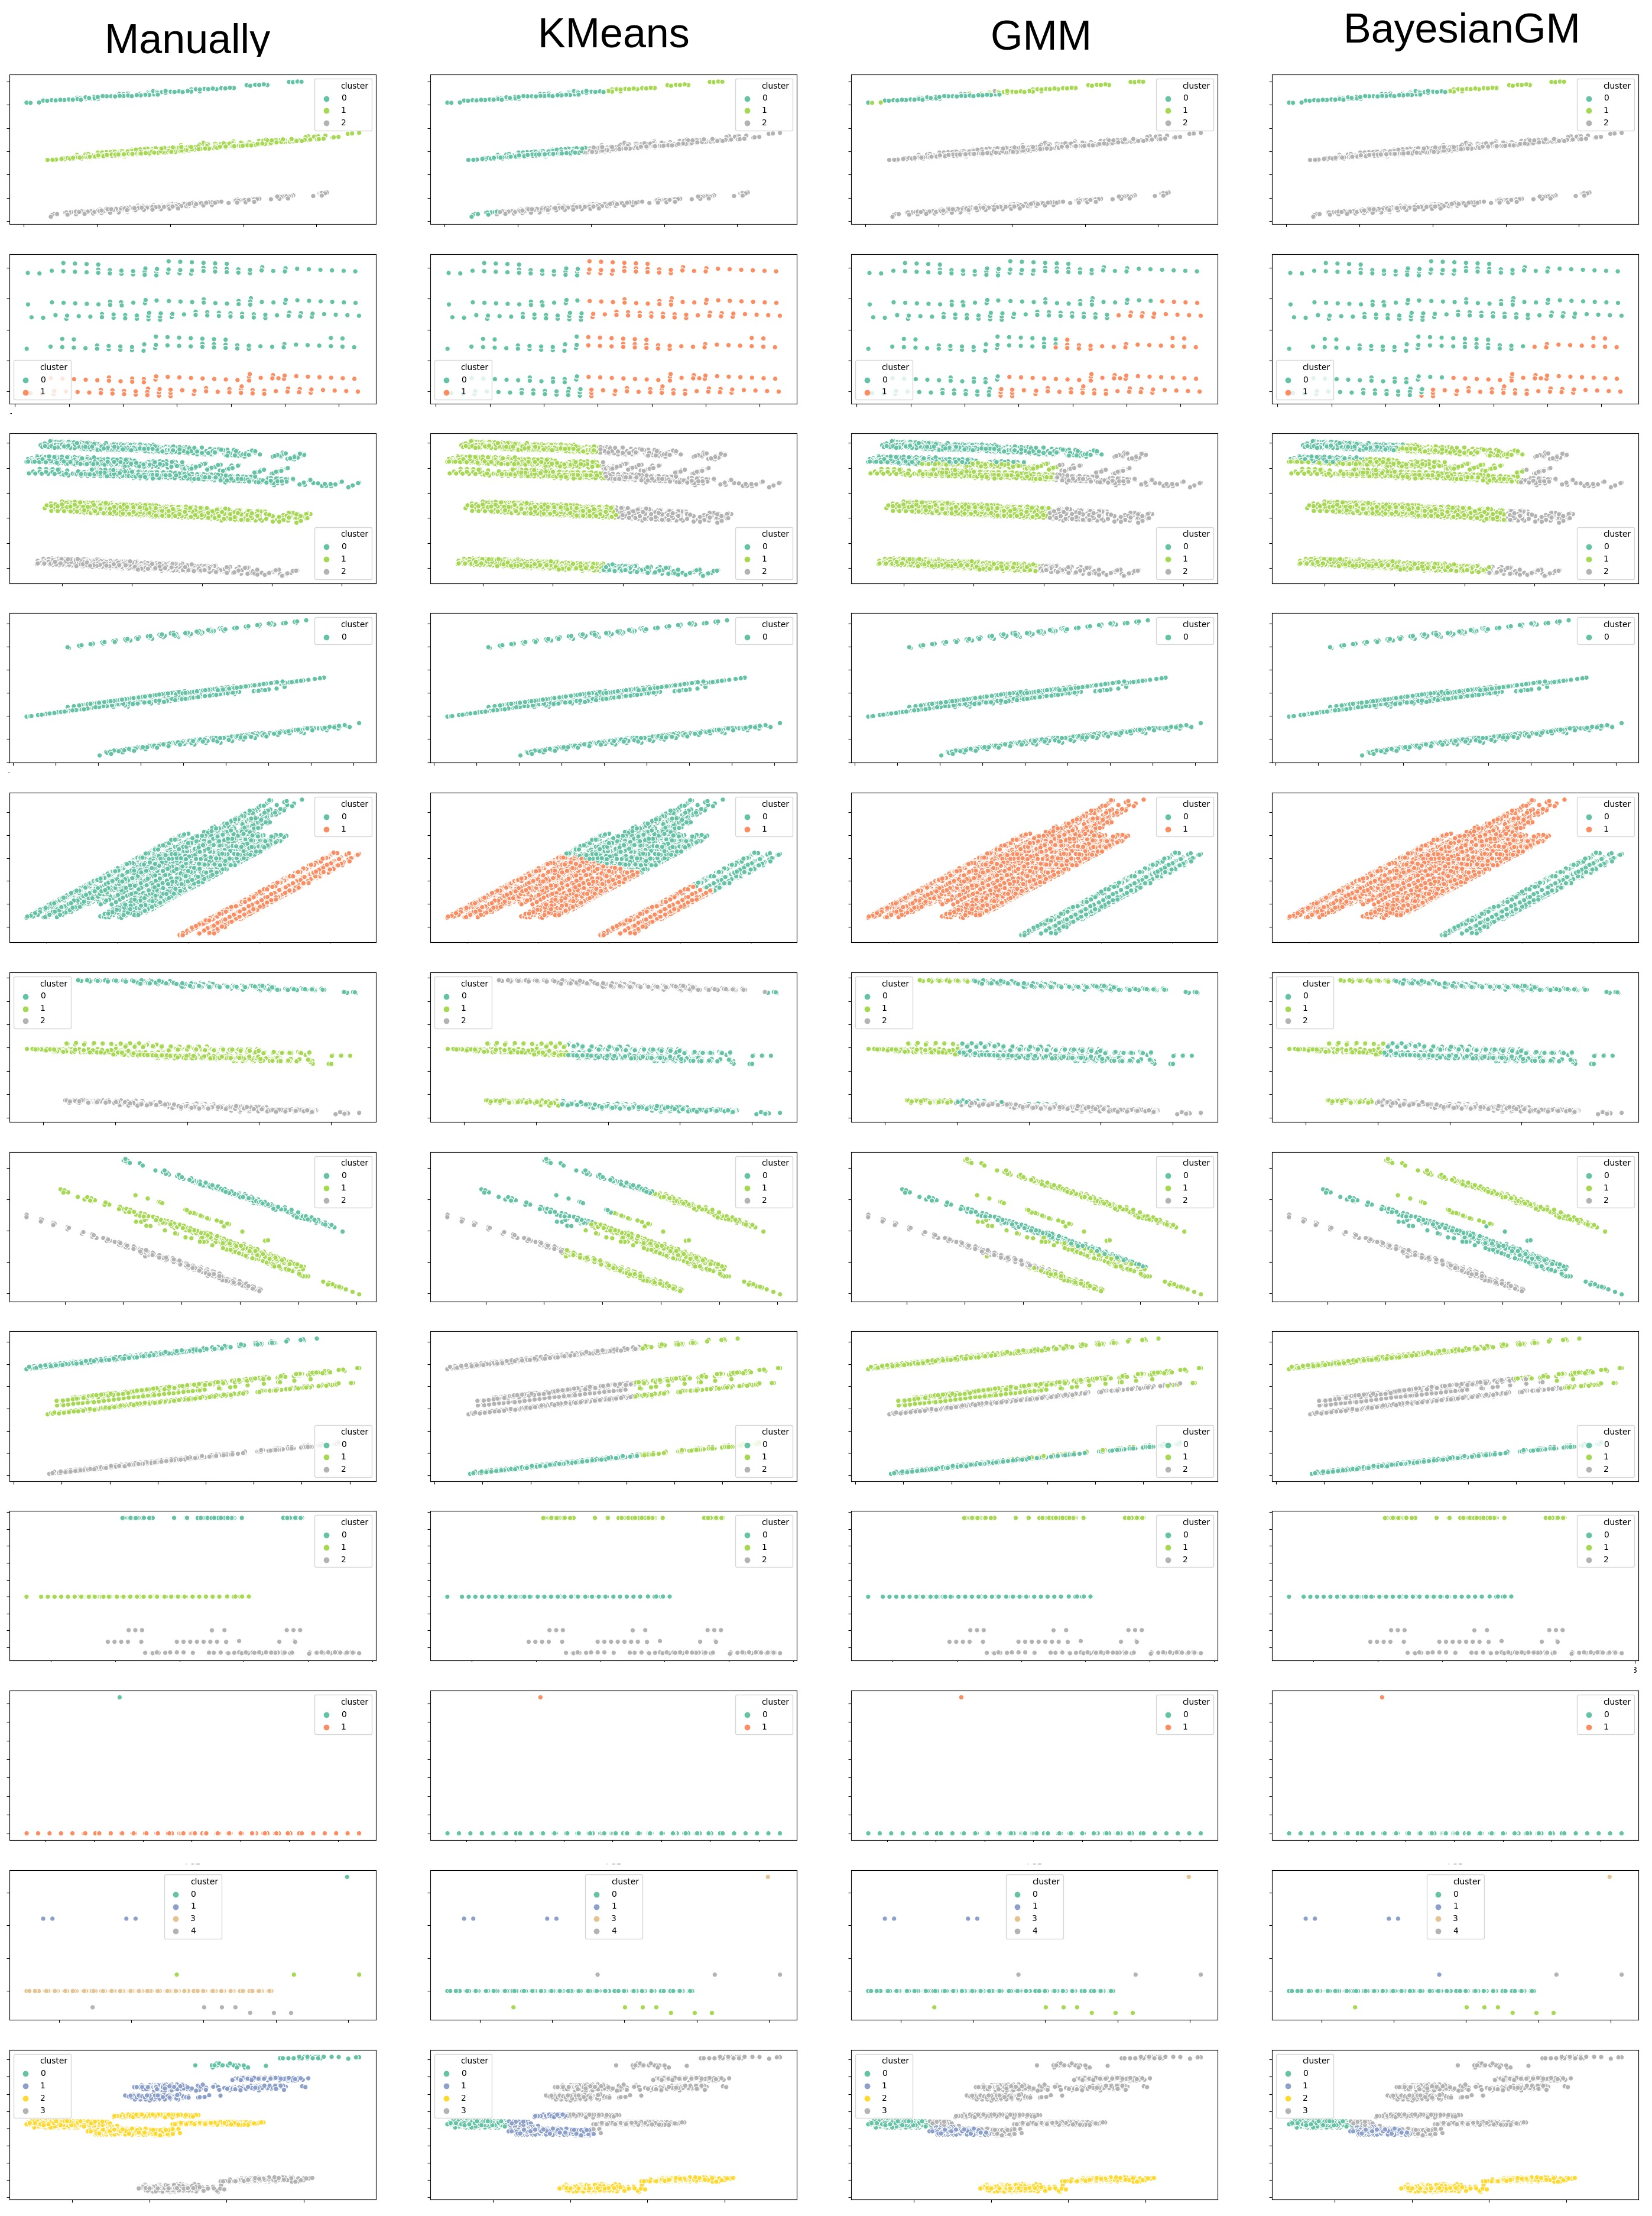
\includegraphics[width=\linewidth]{fig/ch3-clustering-studies.png}
   \caption{Results of the clustering on the first two principal components of some studies. Source: Author}
   \label{fig:clustering-studies}
\end{figure}

\section{Experiments}

In this last part of the chapter, it will be discussed about the experiments that were developed to test the clustering in the OT. After the analysis of the clusters, it was formulated two experiments: \textbf{One run for each cluster} (Experiment I) and \textbf{Clusters as features} (Experiment II).

\subsection{One run for each cluster}

The Experiment I consists in using the clustering strategy I and cluster pairing I. A cluster in a portfolio will be matched with its pair on the market, and each cluster, on a study, will generated a run of the OT. After the runs, all of the outputs will be joined into a single one. So, for the user, the interface still the same. But, internally, OT will split the study in N\footnote{N is the number of clusters} smaller studies and then will aggregate the outputs. These modifications can be better understood when looking to the diagram on Figure \ref{fig:one-run-each-cluster}. 

\begin{figure}[h]
   \centering
   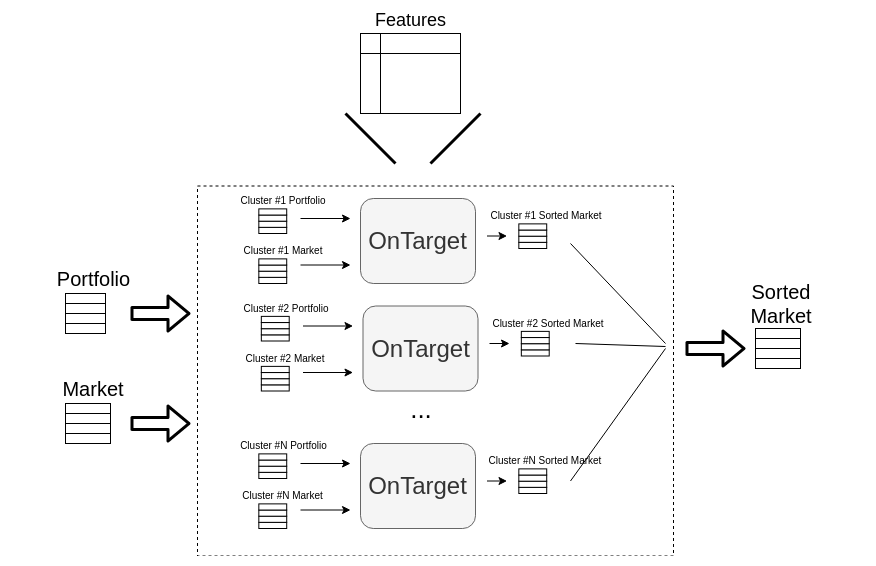
\includegraphics[width=\linewidth]{fig/ch3-one-run-each-cluster.png}
   \caption{Modifications on the OT for the Experiment I. Source: Author}
   \label{fig:one-run-each-cluster}
\end{figure}

To clarify more this idea of the Experiment I, let us take the example of Figure \ref{fig:cluster-strategy}. Since there are two clusters, OT will match the dark blue cluster on the portfolio with its pair on the market, generating one run. Another run will be generated by using the same analogy for the light blue cluster. Then the OT will aggregated both outputs and return as only one sorted market.

Another important modification made on the OT pipeline due to the Experiment I was the definition of a \textbf{minimum size to a study}. There could be cases where, in a portfolio, a cluster has a small number of companies that is not enough for the RS algorithm to create the score. A cluster (sub-run on the OT) must have at minimum:
\begin{itemize}
    \item \textbf{5} companies in the \textbf{portfolio};
    \item \textbf{2} companies in the \textbf{holdout sample}\footnote{in the Experiment I, the holdout set was sampled after the clustering}; and
    \item \textbf{10} companies in the \textbf{market};
\end{itemize}
If one of these is not satisfied, the data is discarded. For example, a study with a portfolio size of 40 and market of 40000, with 3 clusters and the following number of companies in the portfolio/holdout/market: \textbf{Cluster I: 3/1/4000}, \textbf{Cluster II: 20/4/30000}, \textbf{Cluster III: 9/3/6000}. The Cluster I run would be discarded, losing 10\% of the overall study market. Still, there are 36000 companies to search for leads, so it is not a significant loss. Moreover, creating a strategy to allocate these sub-studies' companies that are discarded in other clusters would be cumbersome and it would not be worth it since it is a small percentage of the overall study. Therefore, the discard approach was chosen due to its simplicity.

\subsection{Clusters as features}

The second experiment consists in using the information of the clusters as an extra column in the features table used by the OT. It will not use any of the cluster pairing strategies (it uses the clustering strategy I, though). The Experiment II is much more simple than Experiment I, there is no split on the study, it is not necessary an aggregation of the output, and it is not needed to define a minimum number to a study to run. The information of the clusters is joined with the features table that feed the RS algorithm. Figure \ref{fig:clusters-as-features} shows its simple modification.

\begin{figure}[H]
   \centering
   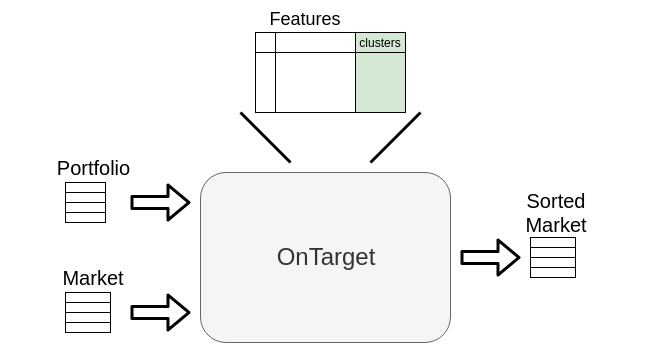
\includegraphics[width=\linewidth]{fig/ch3-clusters-as-features.png}
   \caption{Modifications on the OT for the Experiment II. Source: Author}
   \label{fig:clusters-as-features}
\end{figure}